%----------------------------------------------------------------------------------------
%	CHAPTER 8
%----------------------------------------------------------------------------------------
\chapterimage{ChapterImages/chapter8.png} % Chapter heading image[cite: 1]

\chapter{Processes in Linux and Process Scheduling} %[cite: 1]
\label{ch:processes} %[cite: 1]

In multitasking operating systems like Linux, a \textbf{process} is the basic unit of program execution -- every running program, including every shell script from Chapters~\ref{ch:shell1}--\ref{ch:shell3}, forms at least one process the moment it runs. %[cite: 1] 
The operating system uses mechanisms such as the Process Control Block (PCB), process states, context switching, scheduling, and a handful of system calls to manage these processes. %[cite: 1]

\section{What is a Process and What Components Does It Have?} %[cite: 1]
A process is a representation of a running program, with its information stored in a structure called the PCB. %[cite: 1] 
The main components of a process include: %[cite: 1]
\begin{itemize}
    \item \textbf{Program Code:} the executable instructions. %[cite: 1]
    \item \textbf{Program Counter:} the address of the next instruction to execute. %[cite: 1]
    \item \textbf{Registers:} the current state of the CPU for this process. %[cite: 1]
    \item \textbf{Memory Address Space:} including sections such as Text (code), Data (static data), Heap (dynamic data), and Stack (local variables and function calls). %[cite: 1]
\end{itemize}
The operating system uses this information to manage processes: pausing or resuming them, and switching between multiple processes running on the same CPU. %[cite: 1]

\section{Process Control Block (PCB)} %[cite: 1]
The PCB is a data structure the operating system uses to store information about each process. %[cite: 1] 
Its most important components are listed in Table~\ref{tab:pcb}. %[cite: 1]

\begin{table}[h!]
\centering
\small
\renewcommand{\arraystretch}{1.3}
\begin{tabular}{|>{\raggedright\arraybackslash}p{4cm}|>{\raggedright\arraybackslash}p{9cm}|}
\hline
\textbf{PCB Component} & \textbf{Description} \\ \hline
PID & Unique process identifier (Process ID). \\ \hline
PPID & Parent process identifier (Parent Process ID). \\ \hline
Process State & States like Running, Ready, or Blocked. \\ \hline
Memory Management Info & Pointers to memory sections (Text, Data, Heap, Stack). \\ \hline
I/O Info & Input/output status, open files, and devices. \\ \hline
\end{tabular}
\caption{Main Components of a Process Control Block (PCB)}
\label{tab:pcb}
\end{table} %[cite: 1]

The PCB plays a key role in process management: the operating system uses it to save a process's state when switching away from it, and to restore that exact state later when the process runs again. %[cite: 1]

\section{Process States} %[cite: 1]
A process moves through several distinct states over its lifetime. %[cite: 1] 
Figure~\ref{fig:process-states} shows the standard transitions between them. %[cite: 1]

\begin{figure}[h]
    \centering
    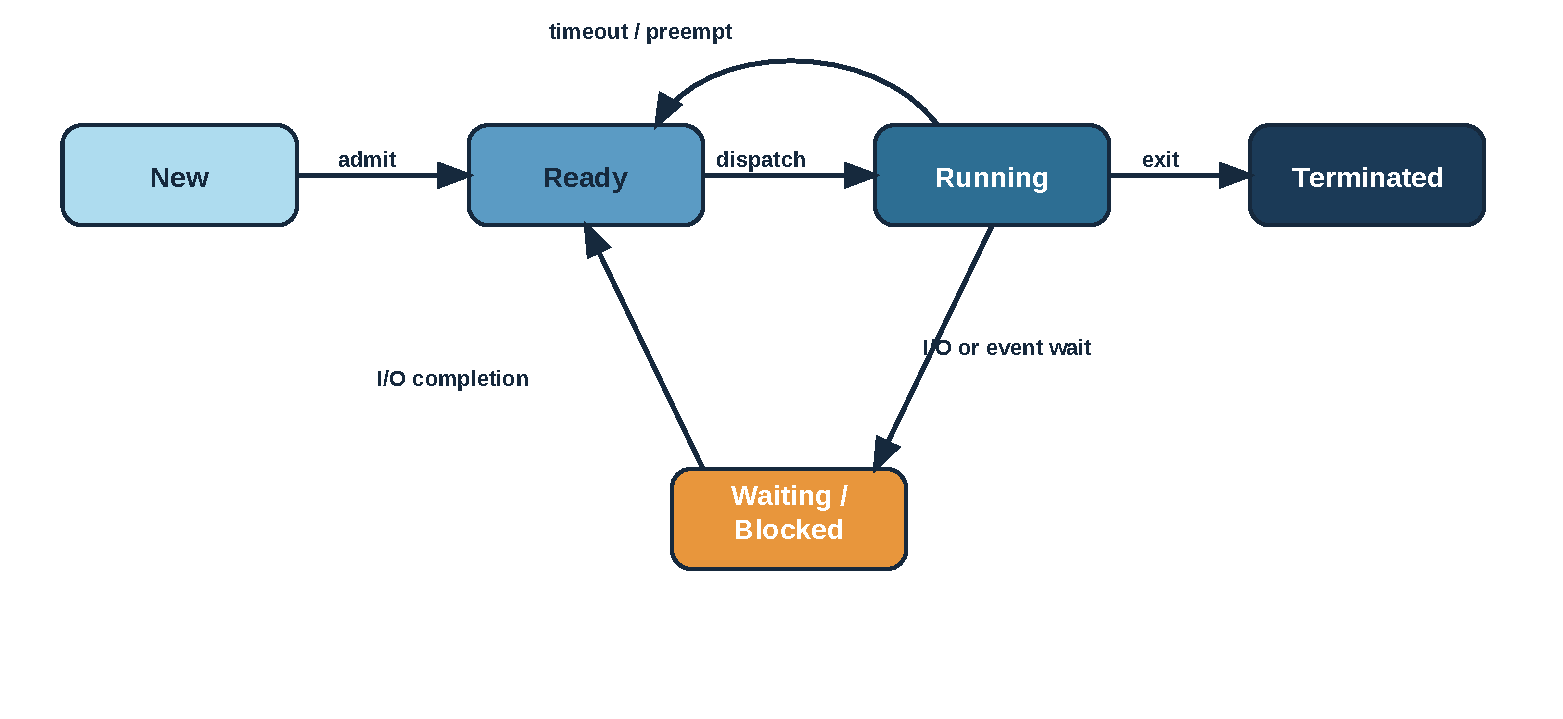
\includegraphics[width=\textwidth]{Images/Chapter8/process-states.pdf}
    \caption{Process state transitions: a process moves between these five states as it is created, scheduled, and eventually terminated.}
    \label{fig:process-states}
\end{figure} %[cite: 1]

\begin{itemize}
    \item \textbf{New:} the process is being created. %[cite: 1]
    \item \textbf{Ready:} ready for execution, waiting only for CPU allocation. %[cite: 1]
    \item \textbf{Running:} currently executing on the CPU. %[cite: 1]
    \item \textbf{Waiting/Blocked:} waiting for a specific event, such as I/O completion. %[cite: 1]
    \item \textbf{Terminated:} execution has finished and its resources have been released. %[cite: 1]
\end{itemize}
Note that a process can only reach \emph{Running} through \emph{Ready} -- it never goes directly from \emph{Waiting} or \emph{New} onto the CPU. %[cite: 1]

\section{Process Management System Calls} %[cite: 1]
In this section, you will learn about three essential system calls: \texttt{fork()}, the \texttt{exec()} family, and \texttt{wait()}. %[cite: 1]

\subsection{\texttt{fork()}} %[cite: 1]
The \texttt{fork()} function creates a child process by making a complete copy of the calling (parent) process. %[cite: 1] 
Figure~\ref{fig:fork} shows what happens to the two resulting processes. %[cite: 1]

\begin{figure}[h]
    \centering
    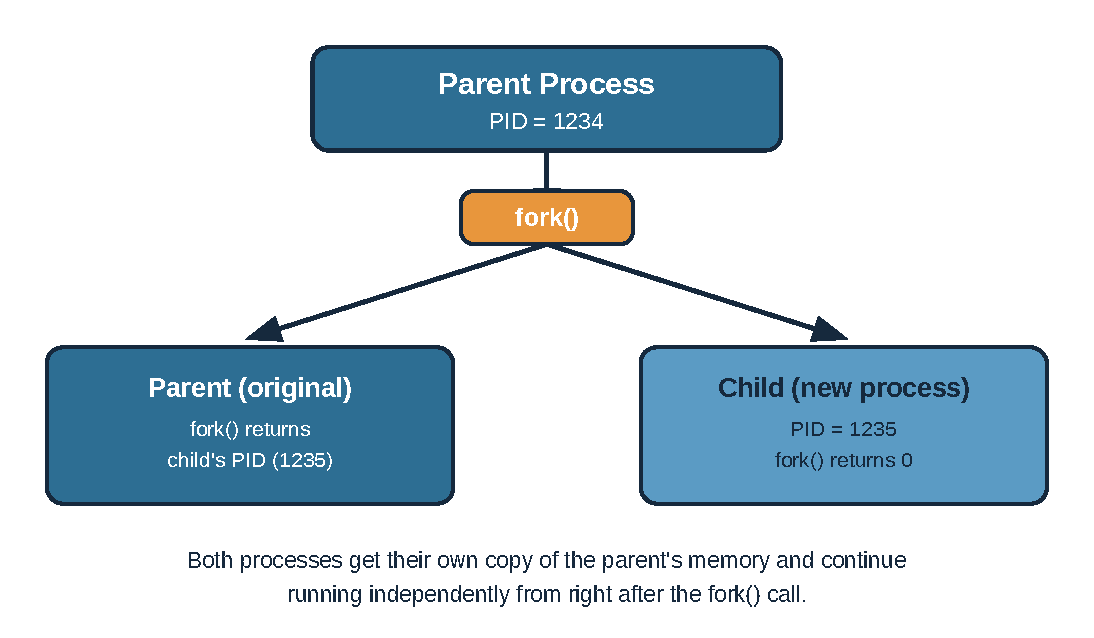
\includegraphics[width=0.85\textwidth]{Images/Chapter8/fork-diagram.pdf}
    \caption{A single call to \texttt{fork()} returns twice: once in the parent, once in the child -- the return value is how each process tells which one it is.}
    \label{fig:fork}
\end{figure} %[cite: 1]

\textbf{Example Code:} %[cite: 1]
\begin{lstlisting}[language=C]
#include <unistd.h>
#include <stdio.h>

int main() {
    pid_t pid = fork();  // Step 1: Call fork() to create a child process.

    if (pid == 0) {      // Step 2: If pid == 0, we are in the child.
        printf("Child Process: PID = %d\n", getpid());
    } else if (pid > 0) {  // Step 3: If pid > 0, we are in the parent.
        printf("Parent Process: PID = %d, Child PID = %d\n", getpid(), pid);
    } else {             // Step 4: If fork() fails (pid == -1), handle error.
        perror("fork failed");
    }

    return 0;            // Step 5: End the program for both processes.
}
\end{lstlisting} %[cite: 4]

\textbf{Compilation and Execution:} %[cite: 1]
\begin{enumerate}
    \item Compile: \texttt{gcc fork\_example.c -o fork\_example} %[cite: 1]
    \item Run: \texttt{./fork\_example} %[cite: 1]
\end{enumerate}

\textbf{Sample Output:} %[cite: 1]
\begin{lstlisting}[language=Terminal]
Parent Process: PID = 1234, Child PID = 1235
Child Process: PID = 1235
\end{lstlisting} %[cite: 1]

\textbf{Step-by-Step Explanation:} %[cite: 1]
\begin{itemize}
    \item \texttt{fork()} is called, creating the child process; the parent's memory space is copied. %[cite: 1]
    \item In the child, \texttt{fork()} returns \texttt{0}, so the child's branch of the code runs and prints the child message. %[cite: 1]
    \item In the parent, \texttt{fork()} returns the child's PID, so the parent's branch runs and prints the parent message. %[cite: 1]
    \item If an error occurs (e.g.\ a resource shortage), \texttt{fork()} returns a negative value and \texttt{perror} displays the error. %[cite: 1]
    \item Both processes continue independently from that point on; the order of their output can vary, since it depends on how the scheduler interleaves them. %[cite: 1]
\end{itemize}

\subsection{\texttt{exec()} Family} %[cite: 1]
The \texttt{exec()} family replaces the calling process's own code and data with a new program. %[cite: 1] 
The PID stays the same -- only what that PID is running changes. %[cite: 1]

\textbf{Example Code:} %[cite: 1]
\begin{lstlisting}[language=C]
#include <unistd.h>  // For execvp()
#include <stdio.h>

int main() {
    // Step 1: Define argument array for the new program (here ls -l).
    char *args[] = {"/bin/ls", "-l", NULL};  // NULL is to end the array.

    // Step 2: Call execvp() to replace current process with ls -l.
    execvp(args[0], args);  // If successful, does not return.

    // Step 3: If execvp fails, this code executes.
    perror("execvp failed");
    return 1;
}
\end{lstlisting} %[cite: 3]

\textbf{Sample Output:} the output of the \texttt{ls -l} command (a detailed file listing). %[cite: 1]

\textbf{Step-by-Step Explanation:} %[cite: 1]
\begin{itemize}
    \item Prepare the arguments: \texttt{args[0]} is the program path, and the remaining entries are its parameters. %[cite: 1]
    \item \texttt{execvp} is called: if it succeeds, the current program's code is replaced immediately, and nothing written after the \texttt{execvp} call runs. %[cite: 1]
    \item If it fails (e.g.\ a wrong path), \texttt{execvp} returns and \texttt{perror} shows the error. %[cite: 1] This pattern -- fork, then exec in the child -- is how a shell runs the external commands you type. %[cite: 1]
\end{itemize}

\subsection{\texttt{wait()}} %[cite: 1]
The \texttt{wait()} function lets a parent process pause until one of its children finishes, preventing \textbf{zombie processes}. %[cite: 1]

\textbf{Example Code:} %[cite: 1]
\begin{lstlisting}[language=C]
#include <sys/types.h>  // For pid_t
#include <sys/wait.h>   // For wait()
#include <unistd.h>     // For fork() and getpid()
#include <stdio.h>      // For printf()

int main() {
    pid_t pid = fork();  // Step 1: Create child with fork().

    if (pid == 0) {      // Step 2: In child, perform some task
        printf("Child Process is running: PID = %d\n", getpid());
        // You can add time-consuming work here, like sleep(5);
    } else if (pid > 0) {  // Step 3: In parent, wait for child.
        wait(NULL);        // wait() waits until child finishes.
        printf("Child Process finished. Parent continuing.\n");
    } else {
        perror("fork failed");
    }

    return 0;            // Step 4: End the program.
}
\end{lstlisting} %[cite: 5]

\textbf{Sample Output:} %[cite: 1]
\begin{lstlisting}[language=Terminal]
Child Process is running: PID = 1235
Child Process finished. Parent continuing.
\end{lstlisting} %[cite: 1]

\textbf{Step-by-Step Explanation:} %[cite: 1]
\begin{itemize}
    \item \texttt{fork()} creates the child. %[cite: 1]
    \item The child performs its task (e.g.\ a loop or a \texttt{sleep}). %[cite: 1]
    \item The parent waits with \texttt{wait()}. %[cite: 1] Without it, a child that finishes before its parent reads its exit status becomes a \emph{zombie}: it is done running, but the kernel keeps its PCB around until the parent collects that status. %[cite: 1]
    \item Once the child finishes, the parent continues. %[cite: 1] If the parent dies \emph{before} the child, the child becomes an \emph{orphan} and is adopted by \texttt{init} (PID~1), which will \texttt{wait()} on it instead. %[cite: 1]
\end{itemize}

\textbf{Important Note:} if you suspect a script is leaving zombies behind, look for them with: %[cite: 1]
\begin{lstlisting}[language=Terminal]
$ ps aux | grep Z
\end{lstlisting} %[cite: 1]

\section{Context Switching} %[cite: 1]
A \textbf{context switch} happens whenever the operating system switches the CPU from one process to another. %[cite: 1] The steps are: %[cite: 1]
\begin{itemize}
    \item Save the current process's state into its PCB. %[cite: 1]
    \item The scheduler selects the next process to run. %[cite: 1]
    \item Restore that process's state from its own PCB. %[cite: 1]
    \item Start (or resume) executing the new process. %[cite: 1]
\end{itemize}
Because saving and restoring state takes time that isn't spent running either process, frequent context switching has a real, measurable performance cost -- it's a trade-off the scheduler makes to keep the system responsive. %[cite: 1]

\textbf{Example Code to Observe the Effect:} %[cite: 1]
\begin{lstlisting}[language=C]
#include <unistd.h>  // For fork() and sleep()
#include <stdio.h>   // For printf()

int main() {
    fork();          // Step 1: First fork() - creates 2 processes.
    fork();          // Step 2: Second fork() - now 4 processes (tree structure).

    printf("Process PID: %d\n", getpid());  // Step 3: Each process prints its PID.
    sleep(2);        // Step 4: sleep to simulate time-consuming work and observe switching.

    return 0;        // Step 5: End.
}
\end{lstlisting} %[cite: 2]

\textbf{Sample Output:} %[cite: 1]
\begin{lstlisting}[language=Terminal]
Process PID: 1234
Process PID: 1235
Process PID: 1236
Process PID: 1237
\end{lstlisting} %[cite: 1]

\textbf{Step-by-Step Explanation:} %[cite: 1]
\begin{itemize}
    \item First \texttt{fork()}: produces the parent and child~1. %[cite: 1]
    \item Second \texttt{fork()}: each of those forks again, so the parent produces child~2, and child~1 produces child~3. %[cite: 1]
    \item All 4 processes now print their message; the order depends entirely on the scheduler. %[cite: 1]
    \item Calls to \texttt{sleep} free the CPU, giving the scheduler a natural opportunity to switch to another process. %[cite: 1]
    \item This program is non-deterministic -- the output order can change from one run to the next. %[cite: 1]
\end{itemize}

\section{Displaying Process Structure with \texttt{pstree}} %[cite: 1]
The \texttt{pstree} command visualizes the hierarchical structure of processes in a tree format. %[cite: 1] It helps you see the relationship between parent and child processes -- crucial when working with system calls like \texttt{fork()} that build up process trees. %[cite: 1] By displaying processes as a tree, \texttt{pstree} makes it easy to trace how they were spawned and nested, including their PIDs and (usually) their command names. %[cite: 1]

\subsection{Why Use \texttt{pstree}?} %[cite: 1]
\begin{itemize}
    \item It gives a clear, visual picture of process ancestry: which process spawned which children. %[cite: 1]
    \item It's useful for debugging multi-process programs, spotting zombie or orphan processes, and understanding overall system resource usage. %[cite: 1]
    \item In this lab, it ties directly to the \texttt{fork()} examples above: after running one, you can use \texttt{pstree} to verify the exact process tree your code created. %[cite: 1]
\end{itemize}

\subsection{Basic Usage} %[cite: 1]
The simplest way to use \texttt{pstree} is to run it with no arguments; for more detail, add \texttt{-p} to show PIDs. %[cite: 1]

\textbf{Sample Command:} %[cite: 1]
\begin{lstlisting}[language=Terminal]
$ pstree -p
\end{lstlisting} %[cite: 1]
\begin{itemize}
    \item \texttt{-p}: displays each process's PID alongside its name. %[cite: 1]
    \item This shows the entire system's process tree, starting from the \texttt{init} process (PID~1, usually \texttt{systemd} on modern Linux). %[cite: 1]
\end{itemize}